\documentclass{article}

\usepackage[utf8]{inputenc}
\usepackage{setspace}

\usepackage{amsmath}
\doublespacing

\usepackage{indentfirst}
\usepackage{pdflscape}
\usepackage[left=1in,right=1in,top=1in,bottom=1in]{geometry}

\DeclareUnicodeCharacter{0301}{\'{e}}

\usepackage[font=small,skip=0pt]{caption}
\usepackage[section]{placeins}
\usepackage{titlesec}
\titlelabel{\thetitle.\quad}
\usepackage{authblk}
\usepackage{csquotes}
\usepackage{booktabs}
\usepackage{siunitx}
\newcolumntype{d}{S[ input-open-uncertainty=, input-close-uncertainty=, parse-numbers = false, table-align-text-pre=false, table-align-text-post=false ]}
\usepackage{amssymb}
% \newcolumntype{d}{S[input-symbols = ()]}
\usepackage{float}
\usepackage{dcolumn}
\usepackage[bottom]{footmisc} 
\usepackage[textsize=tiny]{todonotes}
\usepackage{longtable}
\usepackage{array}
\usepackage{multirow}
\usepackage{wrapfig}
\usepackage{colortbl}
\usepackage{pdflscape}
\usepackage{tabu}
\usepackage{threeparttable}
\usepackage{threeparttablex}
\usepackage[normalem]{ulem}
\usepackage{makecell}
\usepackage{xcolor}
\usepackage{afterpage}
\usepackage{graphicx}
\usepackage{subcaption}
\usepackage{bbding}
\usepackage{xargs}
\usepackage{xpatch}
\usepackage{ragged2e}
\usepackage{rotating}
\usepackage[citecolor = blue]{hyperref}
\hypersetup{colorlinks = true, linkcolor = red, urlcolor = teal}

\graphicspath{{~/OneDrive - University of Illinois - Urbana/Research/Projects/Sesmarias Brazil/Figures/01. Maps/}}

\usepackage{bookmark}
\usepackage{todonotes}
\setlength{\marginparwidth}{2cm}

\usepackage[backend = biber, style=authoryear, sorting = nty, maxcitenames=1]{biblatex}

\addbibresource{citations_sesmarias.bib}

\DeclareFieldFormat{citehyperref}{%
  \DeclareFieldAlias{bibhyperref}{noformat}% Avoid nested links
  \bibhyperref{#1}}

\DeclareFieldFormat{textcitehyperref}{%
  \DeclareFieldAlias{bibhyperref}{noformat}% Avoid nested links
  \bibhyperref{%
    #1%
    \ifbool{cbx:parens}
      {\bibcloseparen\global\boolfalse{cbx:parens}}
      {}}}

\savebibmacro{cite}
\savebibmacro{textcite}

\renewbibmacro*{cite}{%
  \printtext[citehyperref]{%
    \restorebibmacro{cite}%
    \usebibmacro{cite}}}

\renewbibmacro*{textcite}{%
  \ifboolexpr{
    ( not test {\iffieldundef{prenote}} and
      test {\ifnumequal{\value{citecount}}{1}} )
    or
    ( not test {\iffieldundef{postnote}} and
      test {\ifnumequal{\value{citecount}}{\value{citetotal}}} )
  }
    {\DeclareFieldAlias{textcitehyperref}{noformat}}
    {}%
  \printtext[textcitehyperref]{%
    \restorebibmacro{textcite}%
    \usebibmacro{textcite}}}

\renewcommand*{\nameyeardelim}{\addcomma\space}

% Makes the authors name bold in the References section:

\def\sectionautorefname{Section}

\title{Land Grants in Colonial Brazil and Long-Term Effects on Development}

\author{Vinicius Okada da Silva\thanks{Contact information: University of Illinois at Urbana-Champaign. Department of Economics, 1407 W. Gregory Drive, David Kinley Hall: Room 126, Urbana, Illinois 61801. E-mail: vo10@illinois.edu}}

\affil{Department of Economics, University of Illinois at Urbana-Champaign}

\date{}

\begin{document}

\maketitle
\thispagestyle{empty} 

\vspace{-.1cm}
\begin{center}
  \textcolor{red}{Latest Update: \today}
  \\
  \href{https://viniokadasilva.github.io/Papers/Sesmarias/02.Draft/02.Second_Draft/Sesmarias_Paper.pdf}{Click here for the Latest Version}
\end{center}
\vspace{.1cm}

\begin{abstract}
  Land access in Brazil has been a key political issue for the past century. The concentration of land in large estates that are often unproductive is argued to be a factor in the low social mobility and inequality of the rural population. However, restricted land access in Brazil has its roots in colonial times. Large plots of land were granted from 1530-1822 through land grants called \textit{sesmarias}. These land grants were often given to people with substantial financial means, restricting land access to most of the population. I contribute to the understanding of colonial land tenure in Brazil by collecting a novel dataset on the location of these land grants alongside a matching procedure, I study the long-term effects of land grants on Brazil's economic development. Preliminary results indicate that the land grants had persistent effects on land concentration, tenure, and usage until the 20th century.
\end{abstract}

\clearpage
\pagenumbering{arabic} 

\section{Introduction}

Brazil has one of the highest levels of land inequality in the world, with ``an estimated 1\% of the population own[ing] 45\% of all land" \parencite{Usaid2016-xs}. 
This issue is compounded by the fact that large agricultural lands in Brazil are often unproductive, with the Brazilian agrarian reform agency indicating that in 2010 ``72\% of all land occupied by large holdings was considered unproductive'' \parencite{Carlson2019-mk}.
The combination of land concentration and low levels of utilization are spread through the economy as it depresses rural wages, keeping those people away from the consumer markets \parencite[p.~1]{De_Oliveira_Andrade1980-xz}.
% However, this is not a recent issue as even in the 1920 census, average land inequality per municipality was already high \parencite{Wigton-Jones2020-ex}. 
However, land inequality is something that has persisted in Brazil ever since its colonization.
As most of the more suitable land had been taken in large estates that were not intensely cultivated \parencite[p.~53]{Mueller1995-gi}. 

[This added to the lack of sharecropping or wage labor].

This paper analyzes the historical colonial causes of land inequality in Brazil, by exploiting geographical and economic variation in the request for land grants, called \textit{sesmarias}.

I exploit the geographical, time, and economic variation of the grants to study their persistent effect in the economic development of

I first describe how the grants themselves were distributed and describe the process of learning that ...

I use a matching algorithm to show that the land grants in Brazil are associated with... . These effects are seen in 1872 and have persisted up to ... 

I then turn to understand what are the mechanisms that are driving the results. 

Given the prominence of land grants in colonial Brazil and the variation on why the land was granted, this paper studies the long-term effects of the role of colonial land assignment in long-term development.  
The paper provides a novel georeferenced dataset of colonial grants in Brazil. 
First, there are no empirical papers studying the direct causes of colonial land distribution in Brazil. 
Previous literature has found negative long-term effects of colonial land usage in Africa and South America \parencites{Dell2010-qt}{Lowes2021-ww}. 
However, there exists evidence that not all land regimes led to negative effects and instead led to economic development, with examples in India and Indonesia \parencites{Banerjee2005-ki}{Dell2019-np}{Ratnoo2023-vw}.  
Other studies have analyzed the effect of land grants in the United States \parencites{Akee2014-uw}{Allen2019-kh}{Smith2023-ip}

This paper also contributes to the understanding of the historical economic development of Brazil by trying to explain the diverging paths in development in each region. 
The land regime and size in each region, as measured by the land grants could have differential impacts on development.
\textcite{Wigton-Jones2020-ex} studies the effects of 1920 agricultural census land inequality and how it still has persisted to the present.
The literature has analyzed how different economic cycles and how immigration have led to differential educational outcomes in Brazil \parencites{Musacchio2014-pq}{Rocha2017-yq}.
Related literature has also analyzed the effect of the Spanish-Portuguese borders in South America, the role of sugarcane, and gold mining in Brazil \parencites{Laudares2022-vy}{Naritomi2012-or}.

\parencite{Dell2010-qt}
\parencite{Sokoloff2000-mb}

\textcite{Ratnoo2023-vw} [Paper about land tenure in India]

\textcite{Albertus2018-bf}


\section{Historical Background}

\subsection{Land Grant Implementation in Brazil}

https://www.taipu.rn.leg.br/a-cidade/

Portuguese presence in Brazil began in 1500, when [...].

Something about the capitanias here [...] 

Quote about how the captains had to give land grants. 

Implementation in the following years.

Portugal tried to implement in Brazil a similar system of land distribution they had successfully done in the Azores and in Portugal.

\textcite[p.~58-59]{Da_Costa_Porto1979-dz} ``Enquanto, no Portugal de D. Fernando, de D.João e de D. Duarte, a distribuição de terra de sesmaria gerou, em regra, a pequena propriedade, no Brasil foi a causa principal do latifúndio"

\parencite{Carlson2019-mk}
``For many Latin American scholars seeking to explain their region’s backwardness in the first half of the  twentieth century, the prevalence of latifundio-dominated agrarian structures was key. The latifundio was  seen  as a  fundamental  impediment  to  economic  development  due  to  its  feudal-like  social  relations,  its   tendency for monocropping, and its negative impact on the formation of domestic markets. However, it  was these scholars’ emphasis on the labor regimes that were characteristic of the latifundio that prevented  them from fully grasping the nature of the problem.''

\parencite{Carlson2019-mk}
``Going back to colonial times, land in Latin America has often been acquired outside of market mechanisms.  This typically occurred through massive land grants from the crown such as the merced, or the sesmaria in  Brazil, or, after independence, through free or low-cost land concessions from national or local governments  (Furtado  2003,  68–80).''

\parencite{Carlson2019-mk}
``These findings are further supported by information from Brazil’s agrarian reform 
agency, which reported in 2010 that more than 50 percent of all large landholdings and 72 percent of all  land  occupied  by  large  holdings  was  considered  “unproductive”  according  to  agency  parameters  (INCRA   2011).''

\parencite{Carlson2019-mk}
``Not only do extensive activities predominate, but land use statistics reveal the low-investment and low- productivity nature of these types of production. On grazing land, for example, if we divide the total number  of animals on large farms by total hectares of pasture, Brazil’s large farms have only 0.65 animals per hectare  of grazing land, while in Peru it is an incredibly low 0.06 animals per hectare (IBGE 2012; INEI 2012).''

\parencite{Carlson2019-mk}
``As Edelman (1992, 22) explains: “the important point is that the dynamics of accumulation are 
radically different than those of classical capitalist development. Rather than investing heavily in improved  technologies,  employing  productive  human  labor,  attempting  to  capture  increased  market  shares,  or   developing linkages with other production processes, latifundistas could become wealthy from harvesting  natural and quasi-natural products of the land.”''

\parencite{Carlson2019-mk} ``Extensive  activities  like  
cattle grazing continued to operate largely as before, as Bicalho and Hoefle (1990, 57) explain for northeast  Brazil: “While the new system of cattle raising uses such technical innovations as planted pasture, pasture  divisions with rotation of use, purchased animal feed, improved breeds and the greater use of vaccines, which  together  with  the  use  of  waged  labour,  satisfy  the  most  demanding  definitions  of  capitalized  agriculture,   the productivity per hectare has not increased significantly. Mere pseudo-modernisation has occurred. The  ranches have all the trappings of being highly productive but the pastures only have one or two steers per  hectare.”"

\textcite{Diegues_Junior1959-ba}

\textcite{Smith1944-oi} ``The only way to distribute the lands was by grants of large tracts as sesmarias''

\textcite{Dean1971-iq} - ``Anyone who claimed to have the means and desire to make use of the land was given a grant, customarily one to three leagues in extent (16.7 to 50.1 square miles).''

\textcite{Simonsen2005-ps} - ``the ones that don't possess sesmarias or can't own land are disowned by the own society they live in"

\textcite[p.~1]{De_Oliveira_Andrade1980-xz}
``The agrarian problem is one of the most serious the country has, because of the great concentration of land ownership and the low level of utilization by the large and medium property owners. A majority of the rural population receives very low wages, which practically puts them outside the consumer market''

\textcite[p.~34-35]{De_Oliveira_Andrade1980-xz} argues that 
``one of the causes that most aggravate the problem [the considerable increase in population, without a corresponding increase in possibilities for employment, is much more a swelling than an orderly growth] is the system of land tenure, dominant since colonization. It tends to contribute to the concentration of property and the lack of guarantees, of written and respected contracts, that would give greater stability to the sharecroppers in the Agreste and the Sertao and to the agricultural workers in the Zona da Mata."

\textcite[p.~36]{De_Oliveira_Andrade1980-xz}
``The concentration of landholdings in the Northeast is a consequence of the essentially commercial character of agriculture there. This character has manifested itself since the start of colonization. Even today, despite the perceptible growth of the middle class and the internal markets, it os predominant. Its control manifests itself in the protection bestowed by the government agencies on the large farms, and in the complete disdain for subsistence farming''

\textcite[p.~113]{De_Oliveira_Andrade1980-xz}
``Extensive cattle raising, with open grazing, did not require much attention or labor. For that reason, the number of slaves in the region was small''

\textcite[p.~119]{De_Oliveira_Andrade1980-xz}
``[The cotton] advantage was a stimulus to the large landowners of the region, since they could increase their profits without modifying their traditional economic activities, and without forsaking cattle raising. Even today one can see that in the Agreste and Sertao cattle raising is the economic activity most associated with the latifundia. The large landowners are always principally cattle raisers and only secondarily farmers. This pattern is broken in the wet areas where climatic conditions are less favorable to cattle raising and where land is almost always in small holdinds''

This paper describes the history of land usage in Brazil and discusses the roles of the sesmarias in it \parencite{Reydon2015-ff}.

\textcite[p.~157]{De_Oliveira_Andrade1980-xz}
``Cattle raising is today, as in the past, the source of great wealth in the Sertao [...] The system of cattle raising on the large fazendas of the Sertao has changed little in recent years''

``The slaves in Brazil were at least partially integrated into society and possessed rights, quite a legal contrast to the plight of the slaves in the United States. Hence their transition from slave to freedman was facilitated. One paramount privilege the slaves enjoyed was their ability to purchase their
own freedom. Blacks, taking advantage of the many Catholic holidays to work on their own, saved money for that purpose. They occasionally formed their own mutual aid societies to facilitate their purchase of freedom.''

\subsection{End of the Land Grants and the 1850 Land Act}

Between 1822 and 1850 there was no clear way on how to obtain lands in Brazil.

1850 Land Law allowed [...]

The first big land reform was in 1964 with the Land Act.

1985 National Agrarian Reform Plan was used.

Land grants were given until 1822, shortly before Brazil's independence.

https://atlas.fgv.br/marcos/caminhos-do-gado/mapas/o-nordeste-da-cana-e-do-gado-no-seculo-17 [IV?]

https://atlas.fgv.br/marcos/movimentos-e-conflitos-sociais/mapas/o-sertao-dos-cangaceiros-1877-1940 [Something About Historical Conflict]

Dutch Brazil ? "dois fatores contribuíram para a penetração do gado para o interior nordestino. O primeiro reside na necessidade de abastecer as áreas açucareiras do litoral com animais para o transporte e de carne para as populações urbanas. O segundo fator foi a presença dos holandeses no século XVII levando os criadores a sair do litoral em direção ao interior devido o temor de perder seus alimentos para os invasores que os requisitavam. Ao fazer isso, os criadores passaram a se estabelecerem em extensões de terra doadas em sesmarias. Um outro fator que também não podemos esquecer é que nesse momento a economia voltava-se para a expansão da empresa comercial canavieira a ponto de a “Carta Régia” de 1701 chegar a proibir a criação de gado até dez léguas da costa" 

``Além deste fator, o autor explicita um condicionante geográfico para a existência desses mercados, pois, as maiores feiras de gado existentes na região se localizam nas cidades que estão exatamente no contato entre o litoral e o sertão.'' \parencite{Galdino_Dantas2008-pw}

``A  cana-de-açúcar foi  plantada,  de  início,  nas sesmarias  e  grandes  proprie- dades  doadas de  500  braças,  até  50  e  200  léguas.  Nos  séculos XVI  e  XVII,  com  os  altos  preços  alcançados  pelo  açúcar,  verificou-se  uma  reação  da  pequena  propriedade,  de  explotação agrícola  limitada,  que,  entretanto,  foi  logo  absorvida  pelos latifúndios. Nos  princípios  do  século  XIX, o panorama da região  açucareira  apresenta-se diferente,  com o  regime da média propriedade, resultante  do parce- lamento  dos  latifúndios,  doados  pelo  excesso  de  terras  devolutas,  pela  escassez  de  colonizadores  ou  pela  repartição  entre  os  herdeiros.  Foi  a  época  em  que  os  engenhos  não  possuíam  mais  do  que  légua  e  meia  ou  duas  léguas .''
\parencite[p.~118]{De_Geografia1970-nk}


``Nos  sertões  da  Bahia,  Pernambuco,  Paraíba,  Rio  Grande  do  Norte,  Ceará,  Piauí, as primeiras estradas foram os  caminhos das boiadas.  Assim  é  que nume- rosas  povoações  - núcleos  de  futuras  vilas  e  cidades  - estabeleceram-15e  às  margens dos rios,  nos lugares onde  êstes ofereciam passagem mais fácil  aos ani- mais,  e  à  beira  dos  caminhos,  nos  pontos  em  que  as  boiadas  paravam  para  descansar.''
\parencite[p.~164]{De_Geografia1970-nk}

\parencite{Panini1990-rj}

Maybe can combine the Sao Paulo ones with the immigration that happened there and contrast.

\subsection{Present Day System}

While the land grants themselves 

\section{Data}

\subsection{Land Grant Dataset}

Given the nature of the grant application, the requirement of a letter to be sent to the governor and approved, a vast number of the letters are [...]

The main source of historical data comes from both a collaboration with the \textit{Sesmarias of the Luso-Brazilian Empire Database} and my own work.\footnote{
  Information on the content of the letters is available at \url{http://plataformasilb.cchla.ufrn.br/}. The georeferencing process was done in collaboration but as a separate project for this paper.}
The database uses archival data from state records, original manuscripts, or other historical data sources to obtain information on the historical concession of land grants in Brazil.\footnote{An example of an original manuscript can be found in \autoref{fig:example_letter_other}, while an example of a transcribed manuscript published by the state archives is available at \autoref{fig:example_letter_sp}.}

When available in the text, information such as the year, the reason for the request, etc. are coded. 
The sesmarias are then georeferenced based on the geographical information present in the text, allowing us to trace them approximately to a geographical point measured as a latitude and longitude coordinate.\footnote{A more in-depth description on how the sources of the letters and how the sesmarias were georeferenced is available in \autoref{app:appendix_data}}\textsuperscript{,}\footnote{More information on the sources used for this project is available in \autoref{app:data_source_appendix}.} \autoref{fig:land_grants_distribution} shows the geographical distribution of the land grants across the states from which I gathered information. 

\subsection{Other Sources}

The main outcome economic variables come from a variety of different sources.
To study the effects of the grants at an earlier time period, I use the 1872 Brazilian Imperial census, which happened only 50 years after the formal ban of land grants in Brazil.
Census data for 1872 is obtained from the Nucleus of Research in Economic and Geographic History from the Federal University of Minas Gerais.\footnote{
  Available at \url{http://www.nphed.cedeplar.ufmg.br/}}
The 1872 Imperial Census contains demographic data at the municipality and parish level and was the last census taken before the abolition of slavery in Brazil. 
Additional work was done to get a novel database at a finer geographical level for the 1872 census.
At that time, the lowest geographical unit at which the census was taken was at the parish level and each municipality included at least one parish.
I then georeference the parishes, allowing me to study the effects with the 1872 census at a smaller geographical unit allowing for better precision of the estimates.\footnote{Distribution of the 1872 parishes alongside the municipality boundaries is available at \autoref{fig:parishes_1872}. For the sample used, I have 469 municipalities and 1,115 parishes. Information on how the parishes were georeferenced is available at \autoref{app:georeferencing_parishes}}\textsuperscript{,}\footnote{More information on the description based on the 1872 census data is available on \autoref{app:variable_construction_1872}}. \autoref{fig:parishes_1872} shows the geographical distribution of the parishes alongside their municipality boundaries. 

To study the persistance of these effects I use data from other censuses from 1970-2010 are obtained from the IBGE (\textit{}).\footnote{Microcensus is available through the IBGE but the data downloaded through the R package \textit{censobr} from \textcite{Pereira2023-qv}}

To study the effect of land usage and tenure I combine satellite data alongside Brazilian Agricultural Censuses. 
Land usage from 1985-2010 is obtained from Mapbiomas \parencite{Souza2020-kb}\footnote{
  Available at \url{https://brasil.mapbiomas.org/en/}}.
Data for current land tenure in 2021 in Brazil is obtained from \textcite{Sparovek2019-dn}.\footnote{
  Available at \url{https://atlasagropecuario.imaflora.org/}}

In addition, I obtain geographical characteristics and shapefiles at the municipality level from a variety of sources. 
Shapefiles for the coast of Brazil, municipality seats, and municipality boundaries from 1872-2010 are obtained from IBGE through \textcite{Pereira2023-qq}.
Information on the slope comes from the European Environment Agency
\footnote{
  Available at \url{https://www.eea.europa.eu/data-and-maps/data/world-digital-elevation-model-etopo5}}, and elevation comes from \textcite{Amatulli2018-gl}.
Data on the maximum amount of calories based on pre-Columbian and post-Columbian crops are obtained from \textcite{Galor2016-ba}. 

\section{Descriptive}

\subsection{Summary Statistics}

Following \textcite{Lowes2021-ww} I show balance on geographical characteristics at the 0.5 x 0.5 (55 x 55km) grid level in [reference to table here].

Summary statistics for the 1872 censuses are available in \autoref{tab:1872summary}. Overall, we can see that municipalities farther from the coast 

\section{Methodology}

[probably cite \parencite{Rocha2017-yq} and compare what he does to us.]

[Can also try the Piabiru for SP \parencite{Barsanetti2021-hp}]

[Or, indigenous tribes \parencite{Barsanetti2023-xq}] -> Also has a very good way of explaining the threats to identification and how I'm dealing with them.

\subsection{Challanges to Identification}

The main concerns about the estimates deal with the endogeneity of the location of the grants. 

%\subsection{Checkerboard pattern}
%Something about the grants past some year needing to have one league between them. 

%``Desde  começos  do  século  XVIII,  as   sesmarias  tinham sido limitadas ao máximo de três léguas separadas por uma devoluta" \parencite[p.~201]{Simonsen2005-ps}

\subsection{Matching}

To study the effects of the land grants I use a propensity score matching procedure to select control municipalities that are similar in geographical characteristics to those that received at least one land grant. In the first step, I estimate the following:

\begin{equation}
  LandGrant_m = X_{m,s} + \mu_s + \epsilon_{m,s}
\end{equation}

The set of variables used to match are: latitude, longitude, mean elevation, mean slope, soil quality for food crops\footnote{Proxied by the measures of \textcite{Galor2016-ba}.}, potential sugarcane output from the FAO, and the distance to the coast.\footnote{In Appendix ? I show that the results are robust to a different set of control variable.} These variables are selected because they are proxies for agricultural output, geographical location, market access, and the main export of Brazil during the colonial times which was sugarcane. For each treated municipality I select one untreated municipality to be its control, which generates the matched sample.

For the matched sample I then estimate the following equation:

\begin{equation}
  Y_{m,s} = LandGrant_m + X_{m,s} + \mu_s + \epsilon_{m,s}
\end{equation}

The assumption for the matched sample is that conditional on the set of controls, the municipalities that received a land grant are as good as random since the control municipalities had similar geographical characteristics. 

The results are found in tables X, Y, and Z. In each Panel, I consider whether the given municipality had any land grants, a land grant pre-1700 and a land grant only post-1700. The 1700 cutoff is chosen due to two historical factors: First, in 1698 it was imposed a limit on the size of the grants to be 3x1 leagues maximum [add citation here]. Additionally, in 1701 there was a ban on livestock grazing within 80km of the coast. The 1700 cutoff, therefore, chooses the combination of the two. Ideally, we would expect that the effects on land usage would change in favor to [add here] and [blah blah blah].

\subsection{Dutch Brazil}

\subsection{Coastal Ban on Livestock}

In 1701, the Portuguese Crown enacted a ban on cattle ranching from 80km of the coast (10 leagues) \parencites[p~.40]{Fausto2014-bh}[p~.198]{Simonsen2005-ps}[p~.460]{Bethell1984-of}. 
The law went into effect after complaints from local farmers that cattle grazing was destroying the sugar plantations in the area. 
In effect that led to reserving the coast to be primarily an agricultural area and allowing the expansion of cattle towards the interiors of Brazil \parencite[p.~216]{Junior1967-jv}.
%``Even the law excluded cattle raising from the ten maritime  leagues which had been laid down as the area reserved for  agriculture''
That led to ``a clear specialization between the two activities'' \parencite{Ribeiro2012-lb}.\footnote{An example of the effect can be seen in the Municipality of Ruy Barbosa and the state of Bahia and Caico in the state of Rio Grande do Norte. Both are described as being created by the cattle expansion that happened because of the 1701 Royal Decree. \parencite{UnknownUnknown-ro}}


Historically, the size of landholdings in the interior of Brazil at this time was extensive. 
As \textcite[p~.41]{Fausto2014-bh} indicates, the need for large lands to allow cattle to roam free led to the creation of large estates in the area, even bigger than those compared to the coast.\footnote{An example of this would be the d'Avila family which owned a large estate in the state of Bahia [...]}
Even with restrictions on the sizes of the land grants taking into effect in 1698, due to the lack of government oversight the  ``sesmarias on which cattle ranches were established sometimes exceeded hundreds of thousands of acres'' \parencite{Bethell1984-of}.
% ``Landholding in the [interior] was truly extensive. Although there was legislation limiting the size of sesmarias to three square leagues, this restriction was simply disregarded. The sesmarias on which cattle ranches were established sometimes exceeded hundreds of thousands of acres"


\parencite[p~.]{Boxer1962-bj}

``Cattle farming was to supply dry beef, leather, and carrying animals to the sugar mills and, later, to the villas that emerged around mining, but was not to mix itself geographically with these other two important export activities from the colonial period, nor with the coffee estates that emerged during the nineteenth century,  when  Brazil was already independent from  Portugal.'' \parencite{Ribeiro2012-lb}.

``It was there that farms measuring thousands of hectares emerged, where cattle found favourable environmental conditions for the multiplication of herds.''\parencite{Ribeiro2012-lb}.


Given the nature of this ban, I exploit the cutoff of 80 km to use a regression discontinuity design to measure the economic effects of this ban. 

First, I provide evidence that [...] In the first-stage I check whether post-1701 we see an increasing number of land grants dedicated to livestock in municipalities farther than 80 km from the coast. 

[Have to think this as an ITT, same with part of the land grants.]

Secondly, using the 1872 I analyze whether or not there were any effects of the coastal livestock ban on the demographics and economic activities at that time.

\footnote{While this setting would be ideal for a Regression Discontinuity Design, the lack of sample size, especially for the early 1872 census results in noisier estimates. Estimations based on it can be found in Appendix ???}

\textcite{Mueller1995-gi} 

"Sesmarias  remained the only way through  which the  Crown granted  land apart from the tolerance  of squatting" 

"In Brazil land was abundant  and did not represent a constraint  for the production  of sugar   Any individual who 
possessed the capital  and slaves to establish a sugar mill could readily obtain a sesmaria  in which to do so   In fact,  in   many instances  it became necessary to have the means to establish a sugar mill  in order to be granted a sesmaria"

"By squatting the settler risked being expelled as the frontier  advanced, yet this was often  far  in the future   Furthermore,  increasingly   through time, there was the possibility that through occupation and cultivation of the land the settler could acquire  property rights, either through  informal  recognition of those rights or through the ex-post granting of a  sesmaria"

[Move this to the appendix]

Historically livestock-raising areas were [...]

\begin{equation}
  Y_{m,s} = \beta \cdot CoastDist_{m,s} + f(D_{m,s})+ \mu_s + X_{m,s} + \epsilon_{m,s}
\end{equation}

For the 1970-2010 census, given that I have information at the individual level I estimate:

\begin{equation}
  Y_{i,m,s} = \beta \cdot CoastDist_{m} + f(D_{m})+ \mu_s + X_{i,m,s} + \epsilon_{i,m,s}
\end{equation}

With the standard errors being clustered at the municipality level. 


Provision of Public goods is the cause for the effects on literacy in 1970 and onwards (?).

Other links:

\url{http://historialuso.an.gov.br/index.php?option=com_content&view=article&id=6191:escravos-de-ganho&catid=2073&Itemid=121}

\url{https://www.nexojornal.com.br/especial/2017/07/07/censo-de-1872-o-retrato-do-brasil-da-escravidao}

“Quando o senhor não tinha uma função para o escravo, ele deixava o escravo ao ganho”, explica o historiador Diego Bissigo. “Ele ia para cidade buscar emprego e o senhor ficava com o salário que o escravo recebesse. É uma forma de uso para o escravo. Assim, ou alugando para outro senhor também.”

"O termo jornaleiro, refere-se geralmente, a um trabalhador que trabalha à "jorna". Isto é, era contratado para trabalhos de pequena duracao temporal, geralmente agricolas, (vindimas, colheitas, poda...) e como tal, pago ao dia (jornada?)."

"Criado de servir era um termo mais aplicado aos empregados que trabalhavam na Casa ou em serviços mais ligados à Casa (Jardim, cavalos, recados, etc.) ."

\parencite[p.~142]{De_Oliveira_Andrade1980-xz}

\subsection{Treaty of Tordesillas}

\subsection{Other}

\subsection{Instrumental Variable - Distance to Salvador and Olinda}

The main ports in the region were... 

The radiation points for cattle were also...

First-stage indicates that ...

\section{Results}

\subsection{Matching}

\subsection{Human Capital Accumulation}

Following \parencite{Galor2009-bc} I test whether there are associated effects of land concentration on education and human capital accumulation [Something to test].

\section{Heterogeneity}

\subsection{Regional Variation}

The effects between the Northeast and Southeast of Brazil [...]

In Table [...] I show that for the 1985 Agricultural census in the Northeast municipalities, the presence of a land grant is associated with an increase in [...]

In Table [...] the effects for the Southeastern states of Sao Paulo and Minas Gerais are [...]

\parencite{Mueller1995-gi}

\subsection{Economic Activity}

\section{Robustness}

In this section explore the heterogeneity of the economic activity. 

\subsection{Coefficient Bounds}

I use the methodology from to estimate how much unobservables could be impacting the main estimates \textcite{Masten2022-bg}.

\subsection{Randomization Inference}

\section{Conclusion}

\clearpage


\xpatchbibmacro{author}{\printnames{author}}{\textbf{\printnames{author}}}{}{}

\printbibliography

\clearpage

\section*{Figures}

\begin{figure}[h!]
  \caption{Land Grant Distribution}
  \begin{center}
     \makebox[\textwidth]			 
     {\includegraphics[width=\paperwidth]{/Users/vinicius/Library/CloudStorage/OneDrive-UniversityofIllinois-Urbana/Research/Projects/JMP/02. Figures/00.Maps/land_grants_distribution_1991.png}}
  \end{center}
  \textit{Notes:} Geographical distribution of the land grants across the states. Municipalities for the 1991 census are highlighted in red. Each point indicates an unique land grant. 
  \label{fig:land_grants_distribution}
\end{figure}

\begin{figure}[h!]
  \caption{1872 Municipalities and Parish Locations}
  \begin{center}
     \makebox[\textwidth]			 
     {\includegraphics[width=\paperwidth]{/Users/vinicius/Library/CloudStorage/OneDrive-UniversityofIllinois-Urbana/Research/Projects/JMP/02. Figures/00.Maps/parishes_1872.png}}
  \end{center}
  \textit{Notes:} Geographical distribution of 1872 parishes alongside 1872 municipality and state boundaries. The states to which I have information on the land grants are highlighted in red. This map shows that several municipalities, especially in the Southeastern states have more than one parish per municipality. The sample increases by using parish-level information instead of municipalities from 337 to 815.
  \label{fig:parishes_1872}
\end{figure}

\begin{figure}
  \caption{Distribution of Land Grants pre- and post- 1701}
  \begin{center}
     \makebox[\textwidth]			 
     {\includegraphics[width=0.85\paperwidth]{/Users/vinicius/Library/CloudStorage/OneDrive-UniversityofIllinois-Urbana/Research/Projects/JMP/02. Figures/00.Maps/land_grant_distribution_1701.png}}
  \textit{Notes:} This figure considers whether or not any part of the municipality was within 80km of the coast.
  \end{center}
  \label{fig:SesmariasDistribution}
\end{figure}

\clearpage

\section*{Tables}

\subsection{Summary Statistics}

\input{/Users/vinicius/Library/CloudStorage/OneDrive-UniversityofIllinois-Urbana/Research/Projects/JMP/03. Tables/summary_1872.tex}

\input{/Users/vinicius/Library/CloudStorage/OneDrive-UniversityofIllinois-Urbana/Research/Projects/JMP/03. Tables/summary_1872_40km.tex}

\clearpage

\subsection{Matching}

\input{~/OneDrive - University of Illinois - Urbana/Research/Projects/JMP/03. Tables/1995_Ag_Census_Matching.tex}

\clearpage

\input{~/OneDrive - University of Illinois - Urbana/Research/Projects/JMP/03. Tables/1970_Matching_Census.tex}

\clearpage

\input{~/OneDrive - University of Illinois - Urbana/Research/Projects/JMP/03. Tables/1995_Matching_Grid.tex}

\clearpage

\appendix

\setcounter{figure}{0}  
\setcounter{table}{0}  

\renewcommand{\thefigure}{A.\arabic{figure}}
\renewcommand{\thetable}{A.\arabic{table}}

\section{Figures}

\begin{figure}[h!]
  \begin{center}
  \caption{Example letter from \textcite{noauthor_1921-qd}}
  \label{fig:example_letter_sp}
  \vspace{3mm}
  \makebox[\textwidth]	
  {\includegraphics[width = 0.6\textwidth]{~/OneDrive - University of Illinois - Urbana/Research/Projects/Sesmarias Brazil/Documents/Sao Paulo/example.png}}
  \end{center}
  \textit{Notes:} Example letter for the state of Sao Paulo, obtained from \textcite[p.~47]{noauthor_1921-qd}. Based on the letter we extract information on the geographical location, alongside year of concession, economic activity, and etc. This letter extends another page which includes more information.
\end{figure}

\begin{landscape}
\begin{figure}[htbp]
  \begin{center}
  \caption{Example original letter alongside its transcribed version}
  \label{fig:example_letter_other}
  \begin{subfigure}[b]{0.5\textwidth}
  \centering
  \vspace{-20cm}
  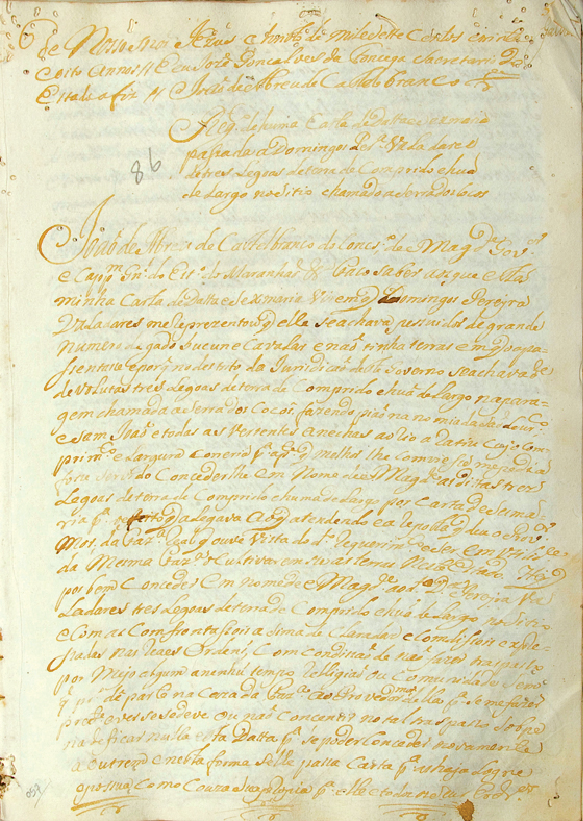
\includegraphics[width = \textwidth]
  {~/OneDrive - University of Illinois - Urbana/Research/Writing/git/Sesmarias/Pictures/0167f614a7c3b3fd38127f1545dbee7c.pdf}
  \end{subfigure}
  \begin{subfigure}[b]{0.6\textwidth}
  \centering
  %\vspace{-7.4cm}
  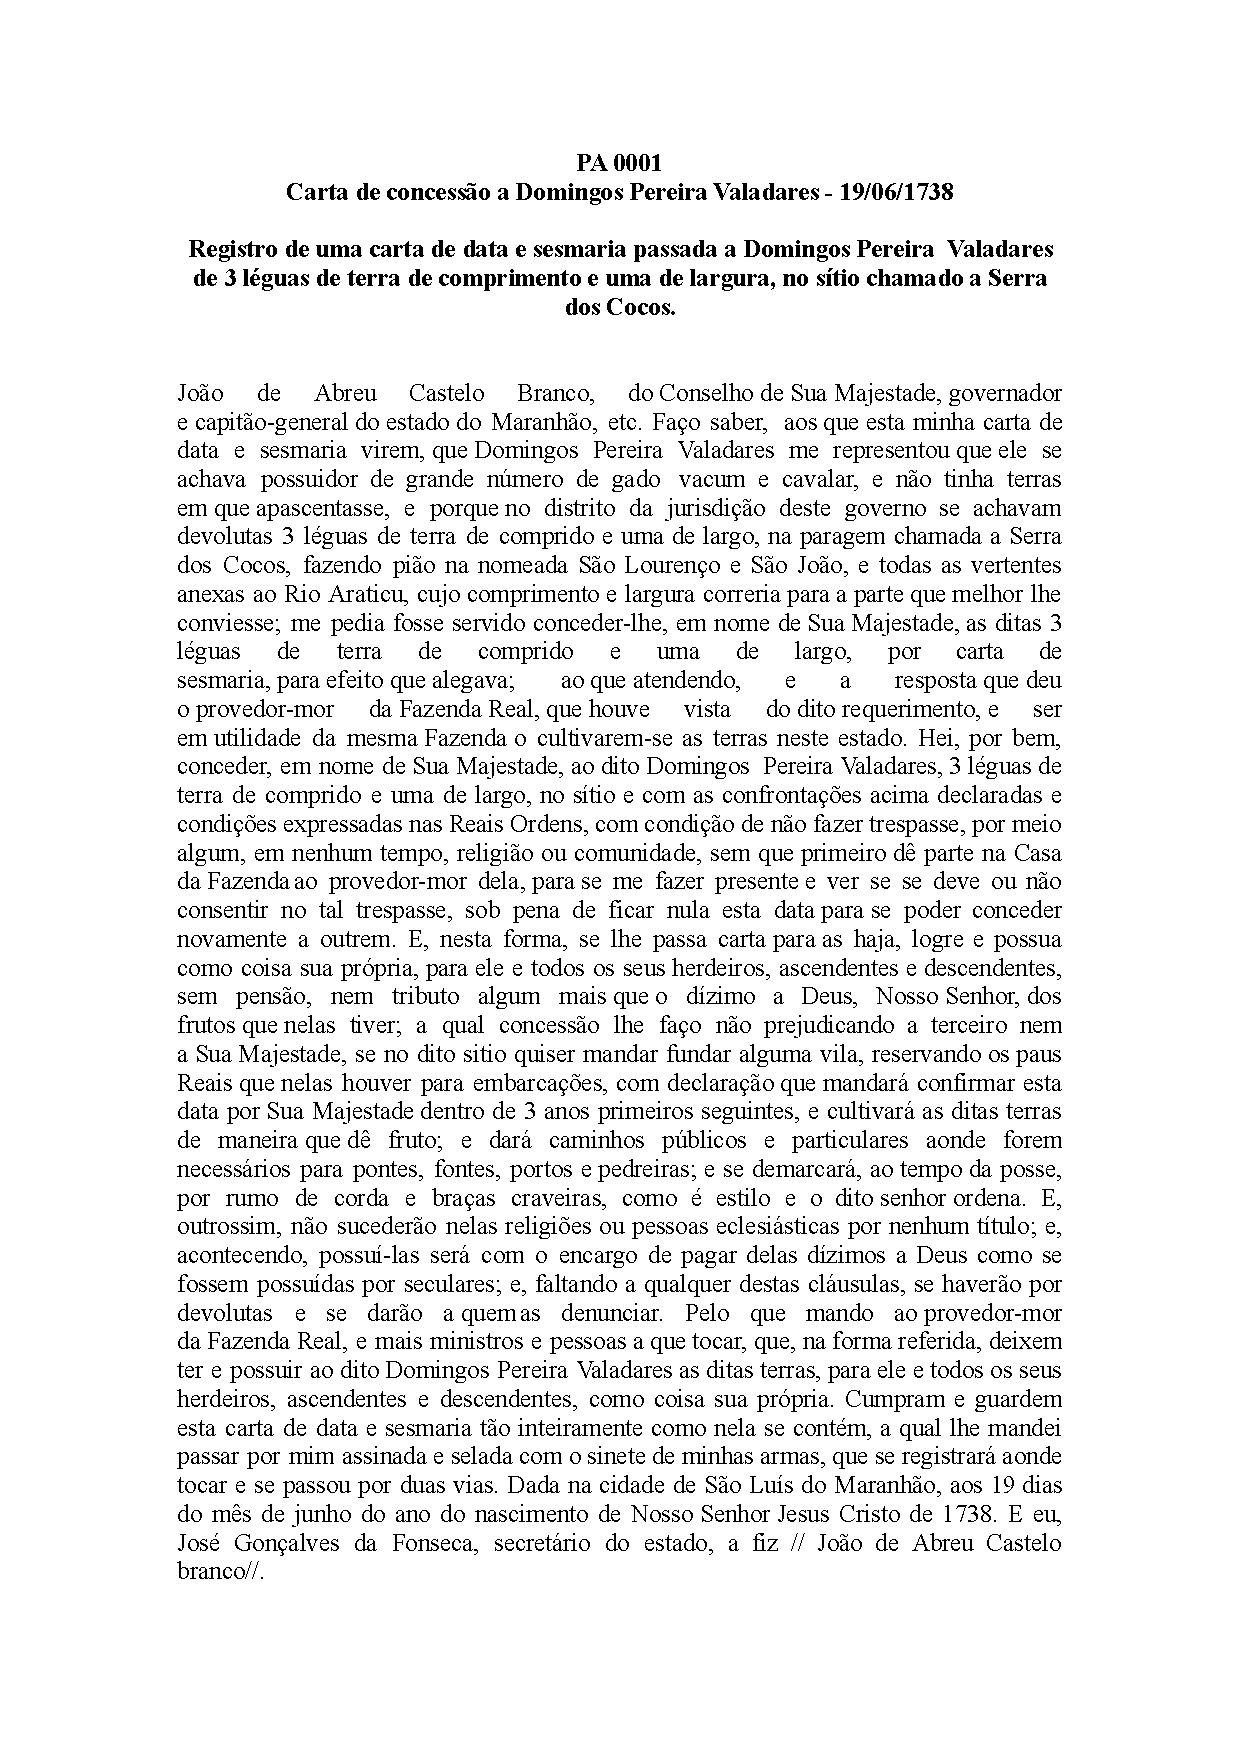
\includegraphics[page = 1, width = \textwidth]
  {~/OneDrive - University of Illinois - Urbana/Research/Writing/git/Sesmarias/Pictures/ea71ea6ac7c5ec3cefa24ded60ac6438.pdf}
  \end{subfigure}
  \end{center}
  \textit{Notes:} Example of an original manuscript and its transcribed version. Obtained from \textit{SILB} with the original source being from ...
\end{figure}
\end{landscape}

\clearpage

[add here the 1872 parishes]

\clearpage

\section{Matching Descriptives}
\label{app:matching_checks}

\begin{landscape}
  \begin{figure}[htbp]
    \begin{center}
    \caption{Example original letter alongside its transcribed version}
    \label{fig:matching_1995}

    \begin{subfigure}[b]{0.3\linewidth}
    \centering
    \includegraphics[scale = 0.5]
    {~/OneDrive - University of Illinois - Urbana/Research/Projects/JMP/02. Figures/00.Maps/Matching_1995_All.png}
    \end{subfigure}

    \hfill

    \begin{subfigure}[b]{0.3\linewidth}
    \centering
    %\vspace{-7.4cm}
    \includegraphics[scale = 0.5]
    {~/OneDrive - University of Illinois - Urbana/Research/Projects/JMP/02. Figures/00.Maps/Matching_1995_1600.png}
    \end{subfigure}

    \hfill

    \begin{subfigure}[b]{0.3\linewidth}
    \centering
    %\vspace{-7.4cm}
    \includegraphics[scale = 0.5]
    {~/OneDrive - University of Illinois - Urbana/Research/Projects/JMP/02. Figures/00.Maps/Matching_1995_1700.png}
    \end{subfigure}

    \end{center}
    \textit{Notes:} Example of an original manuscript and its transcribed version. Obtained from \textit{SILB} with the original source being from ...
  \end{figure}
\end{landscape}

\begin{landscape}
  \begin{figure}[htbp]
    \begin{center}
    \caption{Example original letter alongside its transcribed version}

    \begin{subfigure}[b]{0.75\textwidth}
      \centering
      %\vspace{-7.4cm}
      \includegraphics[scale = 0.75]
      {~/OneDrive - University of Illinois - Urbana/Research/Projects/JMP/02. Figures/00.Maps/Matching_1995_1600.png}
    \end{subfigure}

    \begin{subfigure}[b]{0.75\textwidth}
      \centering
      %\vspace{-7.4cm}
      \includegraphics[scale = 0.75]
      {~/OneDrive - University of Illinois - Urbana/Research/Projects/JMP/02. Figures/00.Maps/Matching_1995_1700.png}
    \end{subfigure}

    \end{center}
    \textit{Notes:} Example of an original manuscript and its transcribed version. Obtained from \textit{SILB} with the original source being from ...
  \end{figure}
  \end{landscape}


\clearpage


\section{Data Source Appendix}
\label{app:data_source_appendix}

Below I describe the sources to which the land grants were compiled from. The states with a $^*$ indicate that the works was done by the researchers at SILB.

\vspace{2mm}

\textbf{Pernambuco$^*$}
\begin{itemize}
\item Documentação Histórica Pernambucana. Recife: Imprensa Oficial, 1954. Vol. 1-2
\item Documentação Histórica Pernambucana: sesmarias. Recife: Secretaria de Educação e Cultura. Biblioteca Pública, 1959. Vol. 1-4
\item Coleção Documentos Históricos Biblioteca Nacional do Rio de Janeiro. Vol. 20-22
\item Arquivo Nacional do Rio de Janeiro. Códice 427
\item Arquivo Nacional do Rio de Janeiro. Códice 155
\item Livro do Tombo do Mosteiro de São Bento de Olinda, Imprensa Oficial - Recife, 1948
\item Livros do Tombo de São Bento. Book 1-3
\item Revista do Instituto Arqueológico, Histórico e Geográfico Pernambucano, 1896.
\item Revista do Instituto Histórico de Goiana, 1871.
\end{itemize}

\textbf{Rio Grande do Norte$^*$}
\begin{itemize}
  \item O Treslado do auto e mais diligências que se fizeram sobre as datas de terras da capitania do Rio Grande, que se tinham dado. Fortaleza: Revista do Instituto do Ceará, 1909, Ano XXIII.
  \item IHGRN - Fundo Sesmarias - Books 1-9
  \item Documentos Históricos da Biblioteca Nacional do Rio de Janeiro..Vol. 23
  \item Documentos Históricos da Biblioteca Nacional do Rio de Janeiro..Vol. 24 Arquivo Nacional Rio de Janeiro, Códice 427
\end{itemize}

\textbf{Bahia$^*$}
\begin{itemize}
  \item Códice 427 - Rio de Janeiro
  \item FREIRE, Felisbello. História territorial do Brasil. Salvador: Secretaria da Cultura e Turismo, Instituto Geográfico e Histórico da Bahia, 1998
  \item DHBN - cartas publicadas na coleção Documentos Históricos da Biblioteca Nacional - DHBN, volumes 13 a 22
  \item  Anais do Arquivo Público do Estado da Bahia - Publicação dos anais do APEB - Anais do Arquivo Público do Estado da Bahia. Volumes 3 e 11
  \item Códice 155 - Rio de Janeiro
  \item Mosteiro de São Bento - Cartas publicadas nos Livros do Tombo do Mosteiro de São Bento  
\end{itemize}

\textbf{Paraiba$^*$}
\begin{itemize}
\item A
\end{itemize}


\textbf{Sao Paulo}
\begin{itemize}
\item \textcite{noauthor_1921-qd} Vols. 1-3 
\end{itemize}

\textbf{Minas Gerais}
\begin{itemize}
\item c 
\end{itemize}

\clearpage

\section{Description of Letters and Georeferencing}
\label{app:appendix_data}
\clearpage

\clearpage

\section{Parish Level Georeferencing}
\label{app:georeferencing_parishes}
\clearpage

\section{Coastal RDD - Results}
\label{app:coastal_rdd}
\clearpage

\section{Data Appendix - 1872}
\label{app:variable_construction_1872}

Below are the definitions of the variables measured for the 1872 census and how they were constructed. Some of the variables are already defined in the census:

\subsection{Base Variables, available by gender and free vs. enslaved:}

\begin{enumerate}
  \item Number of Literate People
  \item Number of People 6-15 Attending/Not Attending/No Information on Schooling
  \item Demographic Information on Race
    \begin{enumerate}
      \item Number of Enslaved People
      \item Number of Pardos
      \item Number of Whites
      \item Number of Blacks
      \item Number of Caboclos
    \end{enumerate}
  \item Number of People not born in the state based on origin: Within Brazil or from another country.
  \item Number of people on types of jobs: Liberal/Manual/Agricultural/Industry/Other Jobs/No Jobs
    \begin{enumerate}
      \item Liberal: Religious men/women, judges, lawyers, notaries, attorneys, justice officials, medics, surgeons, pharmacists, midwives, teachers, public officials, and artists.
      \item Manual or Mechanical: 
      \item Agricultural: Farmers and livestock breeders.
      \item Industry: Manufacturers and merchants.
      \item Other: Military officers, mariners, fishermen, capitalists/owners, \textit{jornaleiros} (workers that are paid based on a working day), domestic workers, and no information
    \end{enumerate}
  \item Number of people by age group.
\end{enumerate}

\subsection{Constructed Variables:}

\begin{enumerate}
  \item Number of Free People Above the Age of 15
  $$ \sum \text{\# Of Free People Above 15} $$

  \item Literacy Rates, following \textcite{Rocha2017-yq}: 
  $$100 \times \frac{\text{\# of Literate Free People}}{\text{\# of Free People Above the Age of 15}}$$

  \item Men Literacy Rates: 
  $$100 \times \frac{\text{\# of Literate Free Men}}{\text{\# of Free Men Above the Age of 15}}$$

  \item Women Literacy Rates: 
  $$100 \times \frac{\text{\# of Literate Free Women}}{\text{\# of Free Women Above the Age of 15}} $$

  \item Total number of children between 6-15
  \begin{equation*}
    \begin{array}{l}
  \text{\# of Free People between the ages 6-15 who attend school} + \\ \text{\# of Free People between the ages 6-15 who do not attend school} + \\ \text{\# of Free People between the ages 6-15 with no information on schooling}
    \end{array}
  \end{equation*}

  \item Percentage of Children between age 6-15 who are attending school:
  \begin{equation*}
    100 \times \frac{\text{\# of Free People between the ages 6-15 who attend school}}{\text{Total \# of Free Children between 6-15}}
  \end{equation*}

  \item Percentage of Boys between age 6-15 who are attending school:
  \begin{equation*}
    100 \times \frac{\text{\# of Free Boys between the ages 6-15 who attend school}}{\text{Total \# of Free Boys between 6-15}}
  \end{equation*}

  \item Percentage of Girls between age 6-15 who are attending school:
  \begin{equation*}
    100 \times \frac{\text{\# of Free Girls between the ages 6-15 who attend school}}{\text{Total \# of Free Girls between 6-15}}
  \end{equation*}

  \item Proportion of Slaves to Free Population:
  $$ 100 \times \frac{\text{\# of Enslaved People}}{\text{\# of Free People}} $$

  \item Proportion of White/Caboclo/Black/Pardo:
  $$ 100 \times \frac{\text{\# of Free People of Certain Race}}{\text{\# of Free People}}$$

  \item Proportion of Internal/Foreign Immigrants:
  $$ 100 \times \frac{\text{\# of Free People of Certain Immigration Category}}{\text{\# of Free People}}$$
  \item Proportion of Teachers per 10,000:
  $$ 10000 \times \frac{\text{\# of Free People working as Teacher}}{\text{\# of Free People}}$$
  \item Proportion of Workers by Labor Market characteristics (as described in the data above):
  $$ 100 \times \frac{\text{\# of Total People in Certain Job}}{\text{\# of Total People}}$$
\end{enumerate}

\end{document}